\documentclass[12pt]{article}

\usepackage{graphicx}
\usepackage{html}
\usepackage{amssymb}
\usepackage{hyperref}

\renewcommand{\familydefault}{\sfdefault}

\setlength{\textwidth} {6.5 true in}
\setlength{\textheight}{9 true in}
\setlength{\hoffset}   {-0.50 true in}
\setlength{\voffset}   {-0.75 true in}

\begin{document}

\begin{latexonly}
\subsection*{The Quadratic Formula}
\end{latexonly}

\begin{itemize}
\item Equations of the form

  \begin{equation}
    \label{eq:quadratic}
    ax^2 + bx + c = 0
  \end{equation}

  \noindent
  are called \textbf{quadratic equations}. The \textbf{quadratic formula}

  \begin{equation}
    \label{eq:qFormula}
    x = -\frac{b}{2a} \pm \frac{\sqrt{b^2 - 4ac}}{2a}
  \end{equation}

  \noindent
  gives the solutions.

\item The $\pm$ in Eq.~2 %\ref{eq:qFormula}
  is an important detail. In general, there are two solutions to a
  quadratic equation. The two solutions are also called the
  \textbf{roots of the equation}.

\item \textbf{Example}

  A ball is tossed directly upward from a height of 2.0~m above the ground
  with an initial velocity of 5.0~m/s. It is subject only to the force
  of gravity while in flight, so it has an acceleration of
  -9.8~m/s$^2$. When does the ball reach a height of 3.0~m? The position
  of the ball as a function of time is given by the equation

  \begin{equation}
    y = y_o + v_o t + \frac{1}{2}a t^2.
  \end{equation}

  \textbf{Solution}

  The equation with the given information is

  \begin{equation}
    3.0~\mathrm{m} = 2.0~\mathrm{m} + (5.0~\mathrm{m/s}) t 
    + (-4.9~\mathrm{m/s}^2) t^2
  \end{equation}

  \noindent
  which in the form of Eq.~1 %\ref{eq:quadratic}
  becomes

  \begin{equation}
    \label{eq:example}
    (-4.9~\mathrm{m/s}^2) t^2 + (5.0~\mathrm{m/s}) t + (-1.0~\mathrm{m}) = 0.
  \end{equation}

  \noindent
  We can identify $a =-4.9~\mathrm{m/s}^2$, $b = 5.0~\mathrm{m/s}$, and
  $c = -1.0~\mathrm{m}$ and apply Eq.~2,%\ref{eq:qFormula},

  \begin{equation}
    t = -\frac{5.0~\mathrm{m/s}}{2(-4.9~\mathrm{m/s}^2)} 
    \pm \frac{\sqrt{(5.0~\mathrm{m/s})^2 - 
        4(-4.9~\mathrm{m/s}^2)(-1.0~\mathrm{m})}}
        {2(-4.9~\mathrm{m/s}^2)}
        = 0.51~s \mp 0.24~s = 0.27~s, 0.75~s.
  \end{equation}

%  \begin{figure}[h!]
    \begin{center}
      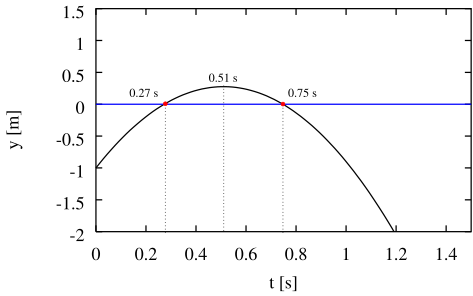
\includegraphics{proj.png}

      Figure 1: The left side of Eq.~5 %\ref{eq:example}
      plotted vs. $t$.
    \end{center}
%    \caption{\label{fig:quad} The left side of Eq.~5 %\ref{eq:example}
%      plotted vs. $t$.} 
%  \end{figure}

  \begin{itemize}
  \item To understand the two solutions, the graph of the left side of
    Eq.~5 %\ref{eq:example}
    shown in Fig.~1 %\ref{fig:quad}
    is helpful. The extreme value of the quadratic occurs at
    $-\frac{b}{2a}$. In the example, the extreme value is at 0.51~s. 

  \item The roots of the quadratic lie $\frac{\sqrt{b^2 - 4ac}}{2a}$ to
    either side of $-\frac{b}{2a}$.  In the example, the two roots of
    the equation lie 0.24~s to either side of 0.51~s.

  \item A graph like this is often helpful in choosing appropriate
    solutions. In the example, both roots of the equation are
    appropriate. The ball reaches a height of 3.0~m twice, once going
    up, and once coming down.

  \end{itemize}

\item \textbf{Special Cases}

  \begin{itemize}
  \item \textbf{Single solution}

    If $4ac = b^2$, then $\sqrt{b^2-4ac} = 0$, and there is only one
    solution, $x=-\frac{b}{2a}$. In the above example, this corresponds to
    0.51~s, the time at which the ball reaches its maximum height. 

  \item \textbf{Complex solutions}

    If $4ac > b^2$, then $\sqrt{b^2-4ac}$ is imaginary (involves $i =
    \sqrt{-1}$). The above example does not have a physically reasonable
    solution corresponding to this situation. (This situation corresponds
    to heights never reached by the ball.)

  \end{itemize}

\end{itemize}

{\footnotesize
  \noindent
  \hrulefill
  
  \noindent
  This work is licensed under the Creative Commons
  Attribution-ShareAlike 4.0 International License: 
  \url{http://creativecommons.org/licenses/by-sa/4.0/}.\\

  \noindent
  L.A. Riley (\texttt{lriley@ursinus.edu}), updated June 2021
}

\end{document}
